\section{Background}
\subsection{How attack happens}
The attack could happen in case of race condition\footnote{Execution of two transactions at the same time with undesirable situation or priority.}, that allows a spender to transfer more tokens than the owner ever wanted. An attacker can execute \textit{transferFrom} function two times by front-running and transfer more token than authorized by \textit{approve} function. According to ERC20 standard:
\begin{enumerate}[label=(\alph*)]
	\item \textit{approve}\footnote{approve(address \textit{\_spender}, uint256 \textit{\_tokens})} function allows \textit{\_spender} to withdraw up to the \textit{\_value} amount of tokens from token pool of the approver. If this function is called again, it has to overwrites the current allowance with the new \textit{\_value}.
	\item \textit{transferFrom}\footnote{transferFrom(address \textit{\_from}, address \textit{\_to}, uint256 \textit{\_tokens})} function grants required rights to the spender (account, wallet or other smart contract) for transferring \textit{\_value} amount of tokens from address \textit{\_from} to address \textit{\_to}.
\end{enumerate}
Usually, \textit{transferFrom} function will be called after \textit{approve} method. The is possible since the \textit{approve} method overrides current allowance regardless of whether spender already transferred any tokens or not. Moreover, transferred tokens are not trackable and only \textit{Transfer}\footnote{Transfer(address indexed \textit{\_from}, address indexed \textit{\_to}, uint256 \textit{\_value})} event will be logged (which is not sufficient in case of transferring tokens to a third parity). Here could be a possible attack scenario:
\begin{enumerate}
	\item Alice allows Bob to transfer N tokens by calling \textit{approve(\_Bob, N)}.
	\item After a while, Alice decides to change Bob's approval from N to M by executing \textit{approve(\_Bob, M)}.
	\item Bob notices Alice’s second transaction before it was mined and quickly sends another transaction that runs \textit{transferFrom(\_Alice, \_Bob, N)}. This will transfer N Alice’s tokens to Bob.
	\item Bob’s transaction will be executed before Alice’s transaction (because of higher transaction fee, miner’s policy or other prioritization techniques) and Bob front-runs Alice’s transaction.
	\item Alice’s transaction will be executed after Bob’s and allows Bob to transfer more M tokens.
	\item Bob successfully transferred N Alice’s tokens and gains ability of transferring another M tokens.
	\item Before Alice notices that something went wrong, Bob calls \textit{transferFrom} method again and transfers M Alice’s tokens by executing \textit{transferFrom(\_Alice, \_Bob, M)}.\newline
\end{enumerate}
\begin{figure}[h]
	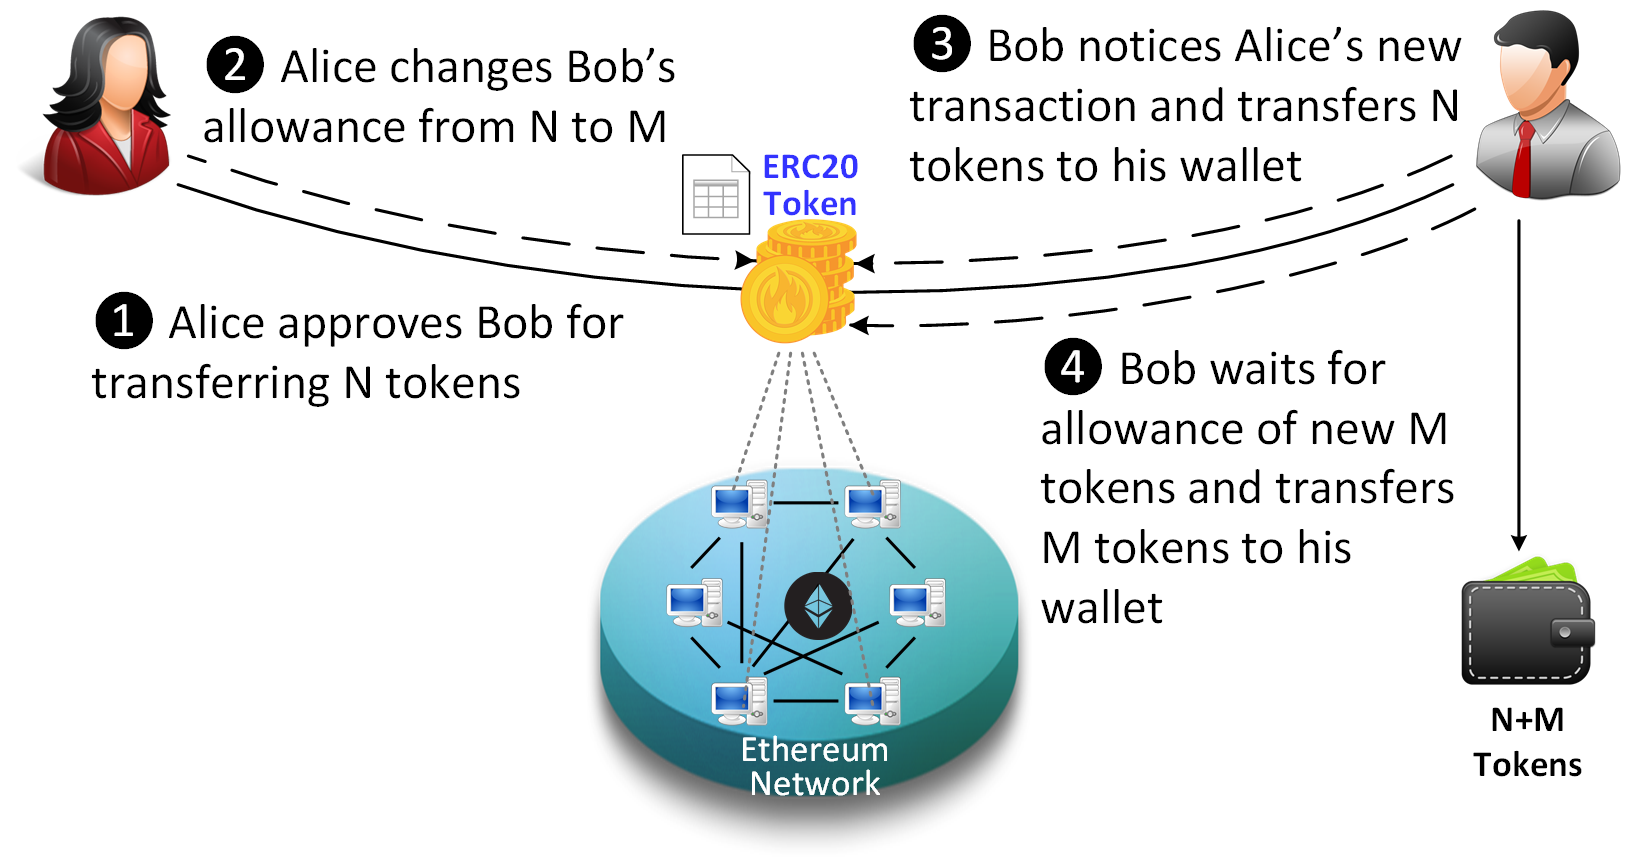
\includegraphics[width=1.0\linewidth]{figures/multiple_withdrawal_02.png}
	\caption{Possible multiple withdrawal attack in ERC20 tokens.}
\end{figure}
Alice attempted to change Bob’s allowance from N to M, but she made it possible for Bob to transfer N+M of her tokens at most, while Alice never wanted to allow so many transfers to be occurred by Bob. It should be noted that the assumption here is to prevent Bob from withdrawing Alice’s tokens multiple times. If he could withdraw N tokens after the initial Alice’s approval, this would be considered as legitimate transfer since Alice has already approved it. In other words, it is Alice responsibility to make sure before approving anything to Bob. 

\subsection{How to mitigate the attack}
We are looking for a solution to prevent multiple withdrawal (N+M) by Bob presuming that Alice has more than N+M tokens in her wallet. ERC20 authors advise owners to change spender allowance from N to 0 and then from 0 to M (instead of changing it directly from N to M). As discussed in "MiniMeToken soultion", changing allowance to non-zero values after setting to zero, will require tracking of transferred tokens by the spender. If we can not track transferred tokens, we would not be able to identify if any token has been transferred between execution of transactions. Although It would be possible to track transferred token through \textit{Transfer} events (logged by \textit{transferFrom}), it would not be easily trackable in case of transferring to a third-party---Alice>Bob, Bob>Carole => Alice>Carole. In short, the goal should be focused on preventing the attacker from transferring more tokens than allowed, instead of adjusting allowance or set it to 0. 

\subsection{What are standard violation constraints}
An important criterion in examining solutions is the standard constraints. We extracted necessary constraints from ERC20 specifications as summarized follows. This constraints must be satisfied by any sustainable solutions:
\begin{enumerate}
	\item Calling \textit{approve} function has to overwrite current allowance with new allowance.
	\item \textit{approve} method does not adjust allowance, it sets new allowance.
	\item Transferring 0 values by \textit{transferFrom} method MUST be treated as normal transfers and fire the \textit{Transfer} event.
	\item Introducing new methods violates ERC20 specifications and it should be avoided for having compatible token with already deployed smart contracts.
	\item Spender will be allowed to withdraw from approver account multiple times, up to the allowed amount.
	\item Transferring initial allowed tokens is considered as legitimate transfer. It could happen right after approval or before changing it.
	\item Race condition MUST not happen in any cases for preventing multiple withdrawal from approver account.\newline
\end{enumerate}